\section{Funktionsweise}

\begin{frame}{Begriffe}
  \begin{Definition}
    Ein \textbf{Repository} ist ein verwaltetes Verzeichnis zur Speicherung und Beschreibung von digitalen Objekten für ein digitales Archiv.\cite{WREP}
  \end{Definition}
\end{frame}

\begin{frame}{Blob}
  \begin{Definition}
    Ein \textbf{Blob} (\glqq \textit{binary large object} \grqq ) ist eine Version einer Datei.
  \end{Definition}
  \begin{itemize}
    \pause
    \item Enthält den Inhalt einer Datei, aber nicht deren Metadaten (Dateiname, Erstelldatum, ...)
    \pause
    \item Ist eindeutig durch den SHA-1 Wert bestimmt (Kollision verschwindend gering)
  \end{itemize}
\end{frame}

\begin{frame}{Tree}
  \begin{Definition}
    Ein \textbf{Tree} enthält Informationen eines Systemordners.
  \end{Definition}
  \begin{itemize}
    \pause
    \item Verweist auf Blobs und weitere (Sub-)Trees.
    \pause
    \item Enthält ebenfalls keine Meta Daten
    \pause
    \item Ist ebenfalls eindeutig durch den SHA-1 Wert bestimmt
  \end{itemize}
\end{frame}

\begin{frame}{Commit}
  \begin{Definition}
    Ein \textbf{Commit} enthält Informationen zu einer Änderung des Repositories.
  \end{Definition}
  \begin{itemize}
    \pause
    \item Verweist auf einen Tree, Autor, ein Datum und weitere Informationen.
    \pause
    \item Hat einen semantischen Sinnzusammenhang
    \pause
    \item Ist ebenfalls eindeutig durch den SHA-1 Wert bestimmt
  \end{itemize}
\end{frame}

\begin{frame}{Commit}
  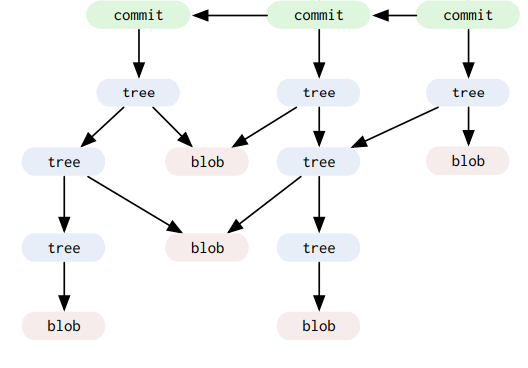
\includegraphics[scale=0.5]{./section/pictures/internes.png}
\end{frame}
